
\section{Test of Consumer Headphones}

\subsection{Purpose}
The purpose of this section is to determine how well the existing consumer headphones available today perform, both on stationary signals but also stochastic speech signals.




\subsection{AAU number list}
\begin{table}[H]
	\centering
	\ra{1.3}
	\begin{tabular}{ c c c } \toprule
		{Item}	& {Description} 						& {AAU-no}. \\ \bottomrule 
		1	&	B\&K Head And Torso Simulator "Henry" Type 4128	& 08453	\\
		2	&	B\&K Ear Simulator Type 4159				& 08453		\\
		3	&	Soundcard RME Fireface 802					& 86838		\\
		4	&	Computer running simulink					& NaN		\\
		5	&	B\&K Sound Calibrator Type 4230				& 08155		\\ 
		6	&	Genelec speaker								& 33990		\\ 
		7	& 	B\&K Microphone Power Supply Type 2804		& 07304		\\
		\bottomrule
		& Tested Headphones & \\
		\bottomrule
	
		8 & Denon AH GC20 & NaN \\
		8 & Bose QuietComfort 15 & NaN \\
		8 & Bose QuietComfort 25 & NaN \\
		8 & B\&O BEOPLAY H8 & NaN \\
			\bottomrule
	\end{tabular}
	\caption{Table over equipment used in test.}
	\label{tab:UsedEquipmentListConsumerHP}
\end{table}



\subsection{Diagram}
\begin{figure}[H]
	\centering
	%\tikzsetnextfilename{OtherBrands}
	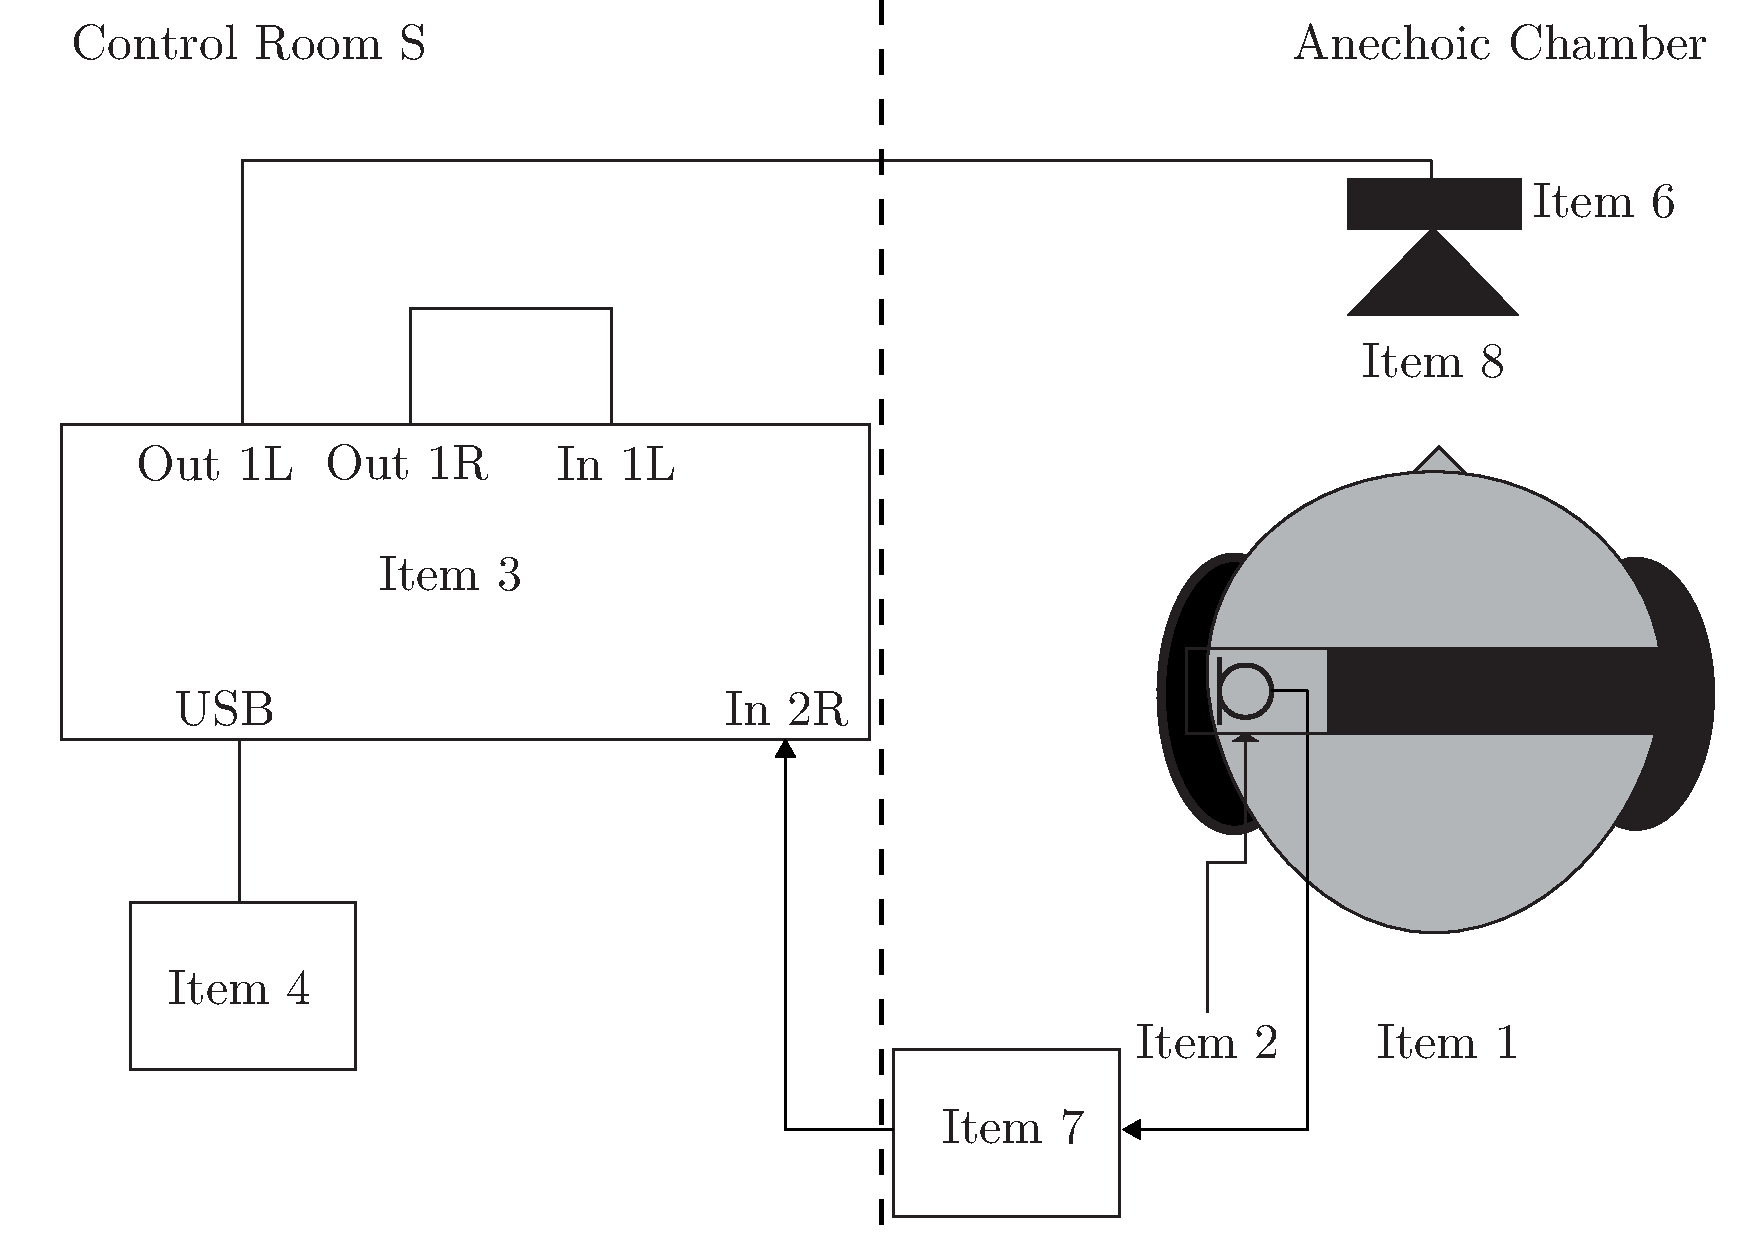
\includegraphics[width=0.8\textwidth]{../Journal/Experiments/TestofConsumerHeadphones/OtherBrandsDiagram.pdf}
	\caption{Diagram of the test set-up.}
	\label{OtherBrandsDiagram}
\end{figure}

\subsection{Settings/Description}
\subsubsection{Control and calibration}
\begin{itemize}
	\item Item 6  is placed 1.6 meters from the Item 1.
	\item Item 2 calibrations are made on the computer using Simulink\textsuperscript{\textregistered}.
	\begin{itemize} 
		\item Calibration is made @ 1 $k$Hz using Item 5 with adapter for Item 2. This should yield a signal of 95.6 dB. The measured intensity in MATLAB\textsuperscript{\textregistered} however was 78.12 so all measurements are multiplied by 7.48 to get a calibrated signal in Matlab\textsuperscript{\textregistered}.
	\end{itemize}
\end{itemize}

\subsubsection{Equipment settings}
\begin{itemize}
	\item This experiment is performed with a sampling rate of, $F_{s}$ = 48 $k$Hz. 
	\item For Item 5 take care to turn on the "inst"-option in the mixing console. The following gain settings are present: 		
	\begin{itemize}
		\item Line level gain is 0 dB
		\item Error Microphones has gain +30 dB
		\item Ref Microphones has gain +48 dB
		\item Speaker Microphones has gain +48 dB
	\end{itemize}
	\item All settings on the computer is set to 0 dBFS
\end{itemize}
	
	
\subsection{Picture}
\begin{figure}[H]
	\centering
	\begin{subfigure}[b]{0.5\textwidth}
		\centering
		%	\tikzsetnextfilename{AttenuationSetup}
		%	
\definecolor{cffffff}{RGB}{255,255,255}

\resizebox {0.4\columnwidth} {!} {
\begin{tikzpicture}[y=0.80pt, x=0.80pt, yscale=-1.000000, xscale=1.000000, inner sep=0pt, outer sep=0pt]
\begin{scope}% layer1
  % text3396
  \path[fill=black,line join=miter,line cap=butt,line width=0.800pt]
    (242.8571,610.2194) node[above right] (text3396) {};

  % rect5654
  \path[draw=black,fill=cffffff,opacity=0.980,miter limit=4.00,line
    width=0.837pt,rounded corners=0.0000cm] (0.0000,492.3622) rectangle
    (460.0000,1052.3622);

  % path5656
  \path[draw=black,dash pattern=on 2.40pt off 0.80pt,line join=miter,line
    cap=butt,miter limit=4.00,even odd rule,line width=0.800pt] (0.0000,482.3622)
    .. controls (460.0000,482.3622) and (460.0000,482.3622) ..
    (460.0000,482.3622);

  % path6121
  \path[draw=black,dash pattern=on 2.40pt off 0.80pt,line join=miter,line
    cap=butt,miter limit=4.00,even odd rule,line width=0.800pt]
    (470.0000,1052.3622) -- (470.0000,492.3622);

  % rect6329
  \path[draw=black,fill=cffffff,opacity=0.980,miter limit=4.00,line
    width=0.800pt,rounded corners=0.0000cm] (220.1005,972.3622) rectangle
    (260.1005,1012.3622);

  % rect6329-8
  \path[draw=black,fill=cffffff,opacity=0.980,miter limit=4.00,line
    width=0.800pt,rounded corners=0.0000cm] (50.3174,692.3748) rectangle
    (90.3174,732.3748);

  % rect6329-8-5
  \path[draw=black,fill=cffffff,opacity=0.980,miter limit=4.00,line
    width=0.800pt,rounded corners=0.0000cm] (370.6172,692.3992) rectangle
    (410.6172,732.3992);

  % rect6329-8-1
  \path[draw=black,fill=cffffff,opacity=0.980,miter limit=4.00,line
    width=0.800pt,rounded corners=0.0000cm] (220.0700,651.8595) rectangle
    (260.0700,691.8595);

  % path6381
  \path[draw=black,fill=cffffff,opacity=0.980,miter limit=4.00,line width=0.800pt]
    (239.6594,819.1820) circle (0.4233cm);

  % path6695
  \path[draw=black,dash pattern=on 2.40pt off 0.80pt,line join=miter,line
    cap=butt,miter limit=4.00,even odd rule,line width=0.800pt] (50.0000,732.3622)
    -- (50.0000,1052.3622);

  % path6697
  \path[draw=black,dash pattern=on 2.40pt off 0.80pt,line join=miter,line
    cap=butt,miter limit=4.00,even odd rule,line width=0.800pt] (0.0000,692.3622)
    -- (220.0000,692.3622) -- (220.0000,1052.3622);

  % path6699
  \path[draw=black,dash pattern=on 2.40pt off 0.80pt,line join=miter,line
    cap=butt,miter limit=4.00,even odd rule,line width=0.800pt]
    (370.0000,732.3622) -- (0.0000,732.3622);

  % text4186
  \path[cm={{0.0,-1.0,1.0,0.0,(0.0,0.0)}},fill=black,line join=miter,line
    cap=butt,line width=0.800pt] (-1049.0592,215.0796) node[above right,rotate=90]
    (text4186) {16 cm};

  % text4186-3
  \path[cm={{0.0,-1.0,1.0,0.0,(0.0,0.0)}},fill=black,line join=miter,line
    cap=butt,line width=0.800pt] (-926.5287,234.3933) node[above right,rotate=90]
    (text4186-3) {15 cm};

  % text4186-1
  \path[fill=black,line join=miter,line cap=butt,line width=0.800pt]
    (252.8320,728.8373) node[above right] (text4186-1) {14 cm};

  % text4186-2
  \path[fill=black,line join=miter,line cap=butt,line width=0.800pt]
    (89.1852,688.5429) node[above right] (text4186-2) {13 cm};

  % text4186-4
  \path[fill=black,line join=miter,line cap=butt,line width=0.800pt]
    (1.3101,746.2242) node[above right] (text4186-4) {12 cm};

  % text4186-0
  \path[cm={{0.0,-1.0,1.0,0.0,(0.0,0.0)}},fill=black,line join=miter,line
    cap=butt,line width=0.800pt] (-914.2587,63.6862) node[above right,rotate=90]
    (text4186-0) {11 cm};

  % text4186-3-8
  \path[cm={{0.0,-1.0,1.0,0.0,(0.0,0.0)}},fill=black,line join=miter,line
    cap=butt,line width=0.800pt] (-781.0693,486.7263) node[above right,rotate=90]
    (text4186-3-8) {10 cm};

  % text4186-3-6
  \path[fill=black,line join=miter,line cap=butt,line width=0.800pt]
    (203.8091,475.7764) node[above right] (text4186-3-6) {17 cm};

  % text4186-2-1
  \path[fill=black,line join=miter,line cap=butt,line width=0.800pt]
    (63.7294,718.4424) node[above right] (text4186-2-1) {A};

  % text4186-2-1-2
  \path[fill=black,line join=miter,line cap=butt,line width=0.800pt]
    (232.8284,677.5307) node[above right] (text4186-2-1-2) {B};

  % text4186-2-1-9
  \path[fill=black,line join=miter,line cap=butt,line width=0.800pt]
    (385.7573,717.3333) node[above right] (text4186-2-1-9) {C};

  % text4186-2-1-6
  \path[fill=black,line join=miter,line cap=butt,line width=0.800pt]
    (233.8228,997.7496) node[above right] (text4186-2-1-6) {D};

  % text4326
  \path[fill=black,line join=miter,line cap=butt,line width=0.800pt]
    (233.0000,826.8622) node[above right] (text4326) {1};

\end{scope}

\end{tikzpicture}}


		\includegraphics[width=\textwidth]{../Journal/Experiments/TestofConsumerHeadphones/Pictures/OtherBrandsSetupBack.jpg}
		\caption{Set-up from the back.}
		%\label{fig:AttenuationSetup}
	\end{subfigure}\qquad
	\begin{subfigure}[b]{0.4\textwidth}
		\includegraphics[width=\textwidth]{../Journal/Experiments/TestofConsumerHeadphones/Pictures/OtherBrandsSetupAngle.jpg}
		\caption{Set-up form an angle.}
		%\label{fig:SetupFront}
		\vspace{2ex}
		\includegraphics[width=\textwidth]{../Journal/Experiments/TestofConsumerHeadphones/Pictures/OtherBrandsSetupSide.jpg}
		\caption{Set-up form the back.}
		%\label{fig:SetupBack}
	\end{subfigure}
	\caption{The test set-up form different angles.}
\label{fig:OtherBrandsPicture}
\end{figure}


\subsection{Procedure}
	\subsubsection{Set-up}
	\begin{enumerate}
		\item Connect cable from Item 3's "Out 1L" to Item 6's "Line in"
		\item Connect cable from Item 3's "Out 1R" to Item 3's "In 1L"
		\item Connect cable from Item 2 to Item 7's "Input"
		\item Connect cable from Item 7's "Output" to Item 3's "IN 2R"
		\item Connect USB-cable from Item 4 to Item 3
	\end{enumerate}

	\subsubsection{Performing Experiment}
	\begin{enumerate}
		\item Open Simulink\textsuperscript{\textregistered} and open and run file "OtherBrands.xls"
		\begin{itemize} 
			\item The simulations outputs a speech signal at 0 dBFS over the span of 20 seconds
			\item The simulation runs for 31 seconds
		\end{itemize}
		\item Rename generated file "GeneratedANC" according to headphone tested, and whether or not ANC was enabled. E.g. "Bose15ANCoff" for Bose QC15 headhpone with ANC disabled.
				\begin{itemize}
			\item[] Perform this experiment for as many headphones as desired.
		\end{itemize}
	\end{enumerate}
	
		
\subsection{Data Extraction}
\begin{enumerate}
	\item Open MATLAB\textsuperscript{\textregistered} and run script "evaluatePerformance.m"
\end{enumerate}

From performing the experiment, a list of files were generated, two for each device tested; one with ANC enabled and one with ANC disabled.
The difference between the enabled and the disabled is plotted on the graph below, for each device tested. The list can be seen below

\begin{itemize}
	\item "DenonANCon.wav"		(Denon AH GC20 w/ ANC)
	\item "DenonANCoff.wav"		(Denon AH GC20 w/o ANC)
	\item "Bose15ANCon.wav"		(Bose QuietComfort 15 w/ ANC)
	\item "Bose15ANCoff.wav"	(Bose QuietComfort 15 w/o ANC)
	\item "Bose25ANCon.wav"		(Bose QuietComfort 25 w/ ANC)
	\item "Bose25ANCoff.wav"	(Bose QuietComfort 25 w/o ANC)
	\item "BOH8ANCon.wav"		(B\&O BEOPLAY H8 w/ ANC)
	\item "BOH8ANCoff.wav"		(B\&O BEOPLAY H8 w/o ANC)
\end{itemize}


\begin{figure}[H]
	\centering
	%\tikzsetnextfilename{OtherBrands}
	\includegraphics[width=0.8\textwidth]{../Journal/Experiments/TestofConsumerHeadphones/OtherBrandsComparison.png}
	\caption{Comparison between Denon AH GC20(Blue), Bose QuietComfort 15(Orange), Bose QuietComfort 25(Yellow), B\&O BEOPLAY H8(Color)  and more to come....}
	\label{OtherBrandsTest}
\end{figure}
FIGURE SHALL BE MADE PRETTY


\subsection{Analysis}
MATH GOES HERE



\subsection{Conclusion}
It was found that bla bla









